%
%  This document contains chapter 3 of the thesis.
%

\chapter{RESULTS}\label{ch:results}
This chapter attempts to answer the questions previously outlined in the
\hyperref[subsec:analysis]{Analysis} section.
Each section is dedicated to exploring one question.
The process used is described in each section though the process usually
consists of using a combination of graphing, One-way ANOVA tests, and
Student's t- or Mann-Whitney U-tests.
All tests are performed with $\alpha = 0.05$ unless otherwise stated.


\section{Lowest Error Voting Mechanisms}\label{sec:lowest-error-voting-mechanism}
Voting mechanisms consolidate the votes of all agents along with their weights
into a final estimate, and so play a pivotal role in the accuracy of a system.
\autoref{fig:voting-mechanisms-comparison} illustrates the population of
squared error for each voting mechanism.

\begin{figure}[htbp]
    \centering
    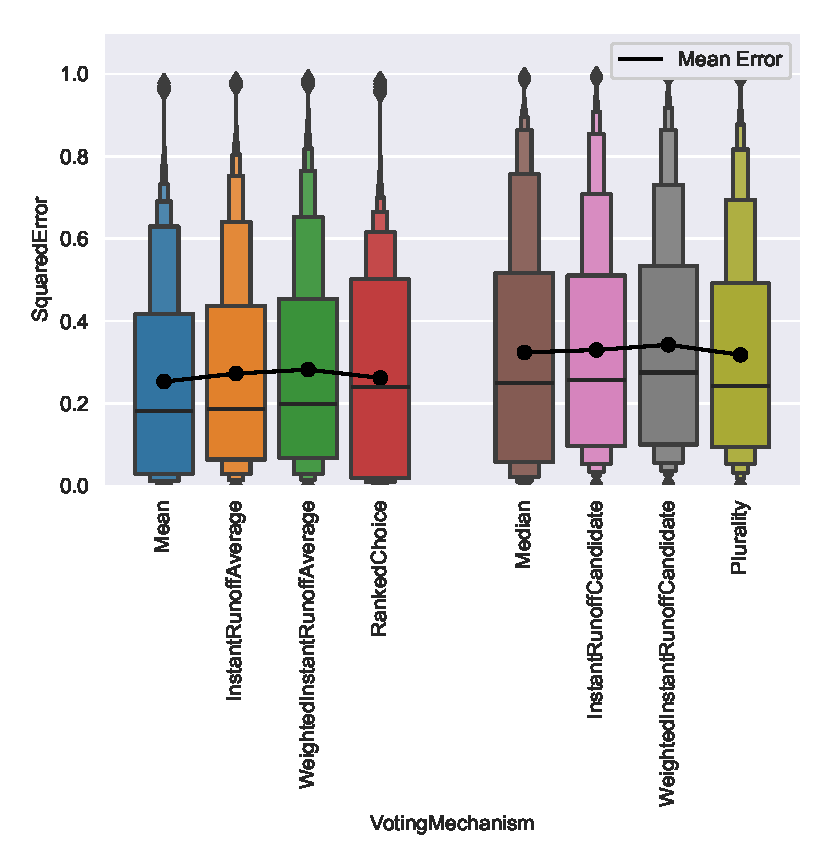
\includegraphics[scale=0.75]
    {./content/figures/voting_mechanisms/voting_mechanisms_comparison}
    \caption{Squared error populations by voting mechanism, with average
    mechanisms on the left and candidate mechanisms on the right.}
    \label{fig:voting-mechanisms-comparison}
\end{figure}

This graph immediately tells us a few things.
First, the squared error seems to be skewed, favoring numbers closer to 0.
This means there is a fairly even spread of estimates, since this is the
pattern one would expect to see from a uniform distribution of estimates.
Interestingly, however, is the majority of most error populations are
somewhere between a uniform distribution of estimates
(\autoref{fig:expected_even_distribution_squared_error}) and a normal
distribution (\autoref{fig:expected_gaussian_distribution_squared_error}).
Indeed, if the estimates are instead graphed as in
\autoref{fig:voting_mechanisms_estimate_distribution}, the distribution of estimates
is more normal than uniform.
This means most mechanisms are better at estimating \truth\ than random chance.

% TODO: Add a table with the mean error for each mechanism

Additionally, while all distributions appear generally close, there appears to be a
slight difference between average and candidate mechanisms.
This can be confirmed by comparing the average mechanisms to the candidate mechanisms
using a Mann-Whitney U-test, with the alternative being the average mechanisms'
squared error is lesser.
Performing such a test results in a p-value of 0.0, far below the $\alpha$ of 0.05.
Since candidate mechanisms can still be useful depending on the situation, both the
best average mechanisms and the best candidate mechanisms will be identified.

Further U-tests were performed, comparing each individual voting mechanism against
every other individual mechanism.
The results of this analysis can be found in
\autoref{fig:all-voting-mechanisms-p-values}, and is further segmented and discussed in
\autoref{subsec:lowest-error-average-mechanisms} and
\autoref{subsec:lowest-error-candidate-mechanisms}.

\subsection{Average Mechanisms}\label{subsec:lowest-error-average-mechanisms}
Average mechanisms, as described in \autoref{subsubsec:average-mechanisms}, work by
averaging the estimates of the system's agents, so it is not too surprising they
result in less error than candidate mechanisms which ultimately output only a single
agent's estimate.
However, they are not all created equally.
This leads us to the question: which average mechanisms generally work best?

To start, an ANOVA test was performed on the average mechanisms.
This produced a p-value of 0, indicating there is very likely a difference between
average mechanisms.
U-tests were then performed to compare each mechanism on its own against each other
mechanism individually, resulting in \autoref{fig:average-mechanisms-p-values}.
The numbers next to the edges are the resultant p-values, where the alternative is
the population is lower than the other.
As is shown by the graph, there is sufficient evidence to reject the null hypothesis
than any of the populations are the same.

\begin{figure}[htbp]
    \centering
    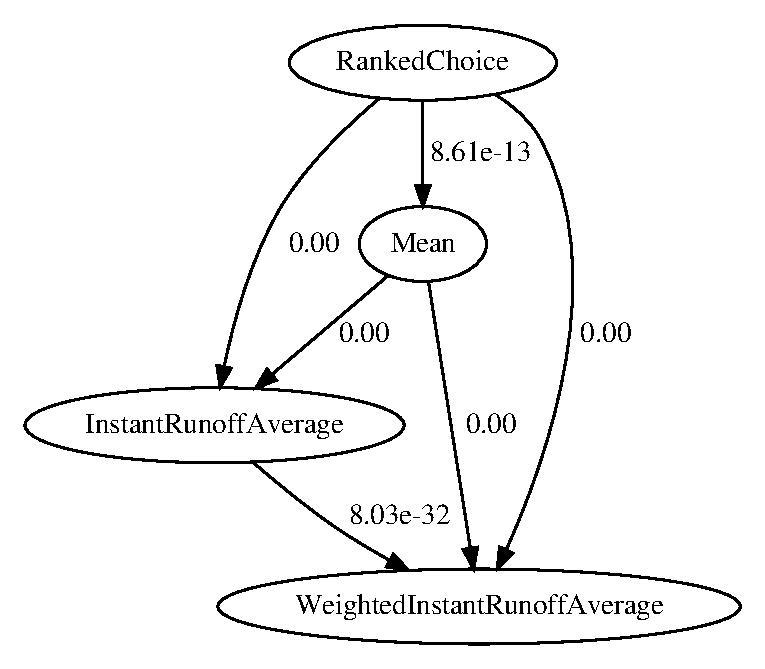
\includegraphics[scale=0.75]
    {./content/figures/voting_mechanisms/average-mechanisms-p-values.gv}
    \caption{The p-values for average voting mechanisms, given the alternative is one
    population is lesser than the other.
    An arrow pointing to another voting mechanism indicates the `from' mechanism
    beats the `to' mechanism.}
    \label{fig:average-mechanisms-p-values}
\end{figure}

In addition, Ranked Choice appears to beat out every other voting mechanism, followed
by Mean beating two, then Weight by Instant Runoff beating one, and finally Averaged
Weighted Instant Runoff beating none.
\begin{samepage}
    This means the rankings of the average mechanisms is as follows:
    \begin{enumerate}
        \item \hyperref[para:avg-ranked-choice]{Ranked Choice}
        \item \hyperref[para:mean]{Mean}
        \item \hyperref[para:avg-instant-runoff]{Weight by Instant Runoff}
        \item \hyperref[para:avg-weighted-instant-runoff]{Averaged Weighted Instant
        Runoff}
    \end{enumerate}
\end{samepage}

\subsection{Candidate Mechanisms}\label{subsec:lowest-error-candidate-mechanisms}
Candidate voting mechanisms are described in \autoref{subsubsec:candidate-mechanisms}.
They work by selecting a single `candidate' and uses its vote as \systemtruth.
While they do not appear to perform as well as average mechanisms, they may be
circumstances where they are required and so they will still be analyzed to determine
which candidate mechanism works best.

An ANOVA analysis was again used to start, which resulted in a p-value of
$2.49e-221$.
This, again, is clearly below $\alpha$, so we can reject the null hypothesis that all
populations are the same.
Following the pattern of analysis in
\autoref{subsec:lowest-error-average-mechanisms}, U-tests where then performed to
identify which mechanisms produced lower error than others.
The p-values can be found in \autoref{fig:candidate-mechanisms-p-values}.

\begin{figure}[htbp]
    \centering
    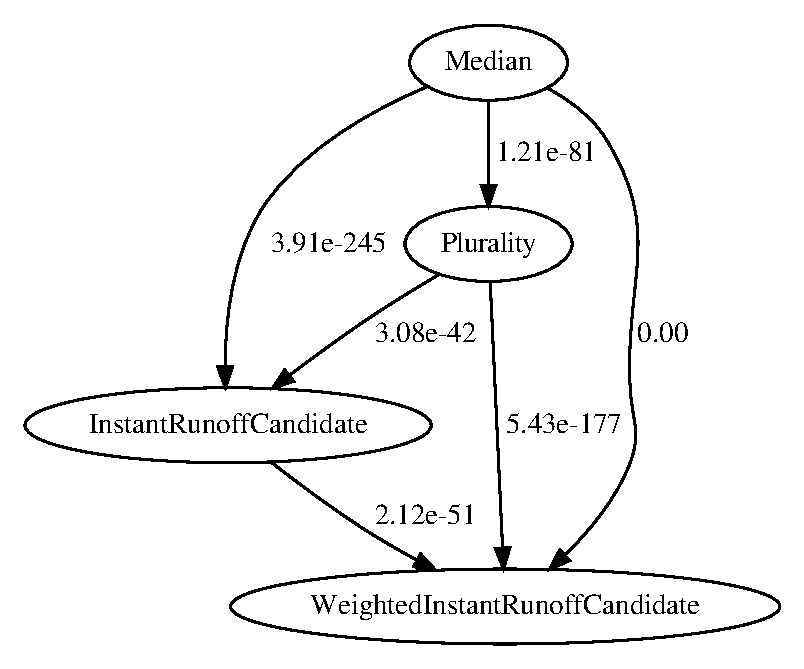
\includegraphics[scale=0.75]
    {./content/figures/voting_mechanisms/candidate-mechanisms-p-values.gv}
    \caption{The p-values for candidate voting mechanisms, given the alternative is one
    population is lesser than the other.
    An arrow pointing to another voting mechanism indicates the `from' mechanism
    beats the `to' mechanism.}
    \label{fig:candidate-mechanisms-p-values}
\end{figure}

While not as many p-values are 0 with the candidate mechanisms, there is still very
strong evidence that each candidate mechanism is not the same as each other.
For the candidate mechanisms, Median appears to be the best, followed
by Plurality, Instant Runoff, and finally Weighted Instant Runoff.
\begin{samepage}
    This means the rankings of the candidate mechanisms is as follows:
    \begin{enumerate}
        \item \hyperref[para:median]{Median}
        \item \hyperref[para:plurality]{Plurality}
        \item \hyperref[para:cand-instant-runoff]{Instant Runoff}
        \item \hyperref[para:cand-weighted-instant-runoff]{Weighted Instant Runoff}
    \end{enumerate}
\end{samepage}


\section{Lowest Error Weighting Mechanisms}\label{sec:lowest-error-weighting-mechanism}
Weighting mechanisms have a direct influence on how voting mechanisms operate in that
they apply weights to the estimates of the proxies.
This naturally has a direct impact on the output of a system.
\autoref{fig:weighting-mechanisms-comparison}

\begin{figure}[htbp]
    \centering
    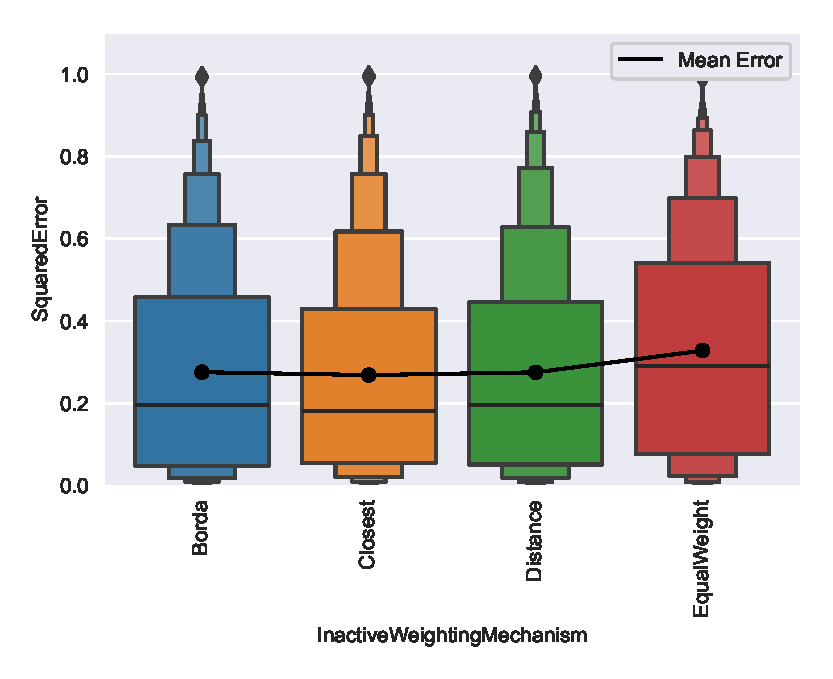
\includegraphics[scale=0.75]
    {./content/figures/weighting_mechanisms/weighting_mechanisms_comparison}
    \caption{Squared error populations by weighting mechanism.}
    \label{fig:weighting-mechanisms-comparison}
\end{figure}

% TODO: Add a table with the mean error for each mechanism

While the mechanisms definitely appear close, there is a visible difference between
the Equal Weight mechanism and the other mechanisms.
This can be confirmed using a series of Mann-Whitney U-tests, resulting in
\autoref{fig:weighting-mechanisms-p-values}.
\begin{samepage}
    This gives us the ordering:
    \begin{enumerate}
        \item \hyperref[para:closest]{Vote for Closest}
        \item \hyperref[para:borda]{Borda}
        \item \hyperref[para:distance-voting]{Distance Voting}
        \item \hyperref[para:equal-weight]{Equal Weight}
    \end{enumerate}
\end{samepage}

\begin{figure}[htbp]
    \centering
    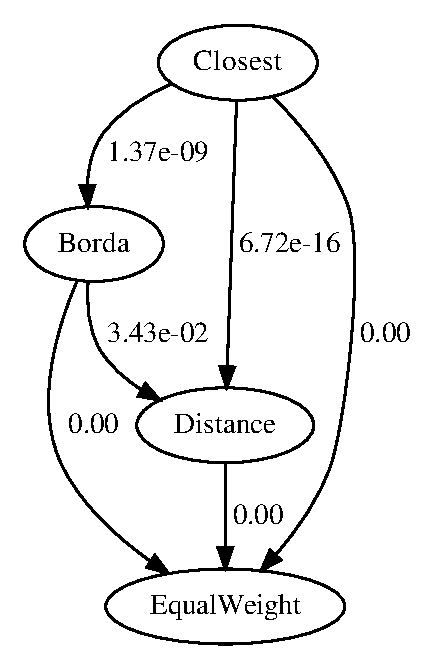
\includegraphics[scale=0.75]
    {./content/figures/weighting_mechanisms/weighting-mechanisms-p-values.gv}
    \caption{The p-values for weighting mechanisms, given the alternative is one
    population is lesser than the other.
    An arrow pointing to another voting mechanism indicates the `from' mechanism
    beats the `to' mechanism.}
    \label{fig:weighting-mechanisms-p-values}
\end{figure}

These results are somewhat surprising in that the simplest method, arguably barring
Equal Weight, appears to produce the best results.
This may be due to the Closest mechanism yielding a lower system-wide weight while
still maintaining an ordering of preferences.
However, this does not necessarily mean the Closest mechanism pairs best with all
voting mechanisms.
This idea is explored in~\fullref{sec:lowest-error-overall-combination}.


\section{Lowest Error Combination}\label{sec:lowest-error-overall-combination}
While the previous sections have explored the lowest error for each voting mechanism and
weighting mechanism regardless of the mechanism it's paired with, this section will
explore the lowest error for each combination of voting and weighting mechanism.

The population of error for each combination is displayed in
\autoref{fig:combined-comparison}, where we see a similar pattern with the voting
mechanisms as what was discussed in \autoref{sec:lowest-error-voting-mechanism}: the
candidate mechanisms tend to be noticeably worse than the average mechanisms.
Additionally, average mechanisms typically produce an error below the weighting
mechanism mean, while candidate mechanisms tend to produce an error that is higher
than the mean.

\begin{figure}[htbp]
    \centering
    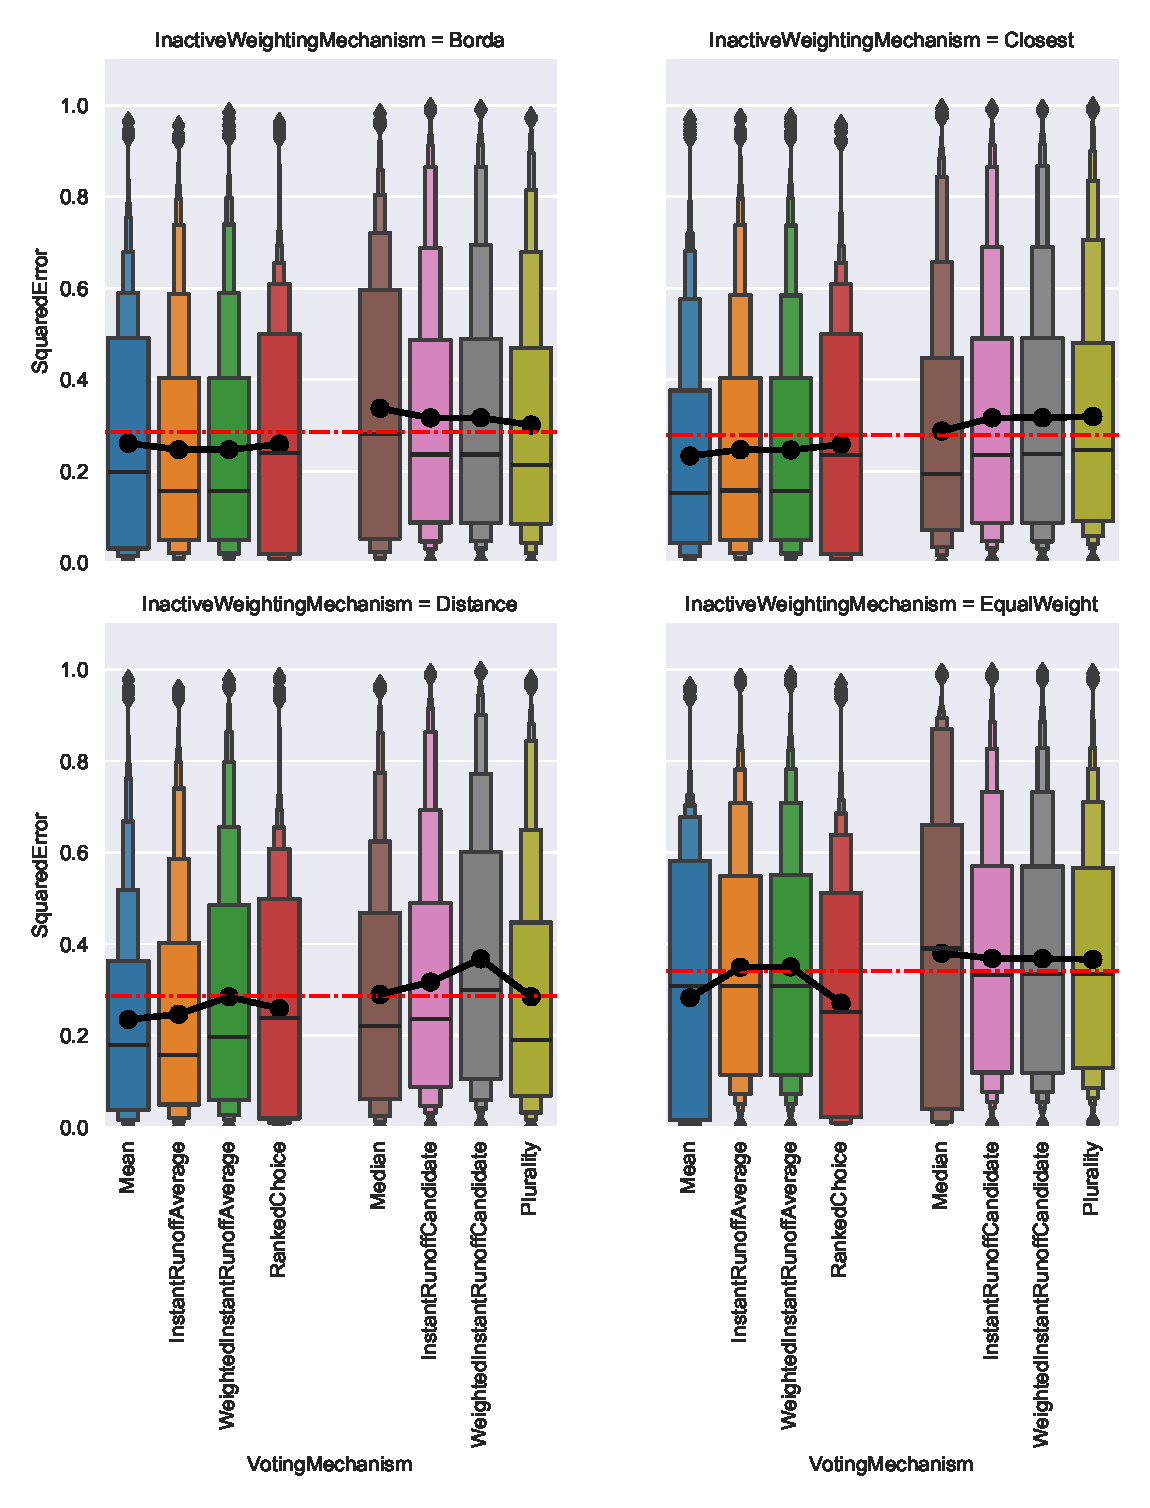
\includegraphics[scale=0.75]
    {./content/figures/combinations/combined_comparison}
    \caption{Squared error populations by combination of mechanisms. The red dashed
    line represents the mean for each weighting mechanism, while the black line with
    dots are the means for each voting mechanism using the weighting mechanism.}
    \label{fig:combined-comparison}
\end{figure}

Using U-tests, we can discover which combinations produce the lowest error.
By counting how many times some combination beats other combinations, we can produce
an over ranking.
The number of times one combination `beats' another by having a lower error is
displayed in \autoref{fig:combined-lesser_counts}, and is further tabulated in
\autoref{tab:combined-overall-rankings}.
From these tests, we can see the averaged easily dominate, with the first candidate
combination being in rank 15, reinforcing the idea that average mechanisms result in
lower error than candidate mechanisms.

\begin{figure}[htbp]
    \centering
    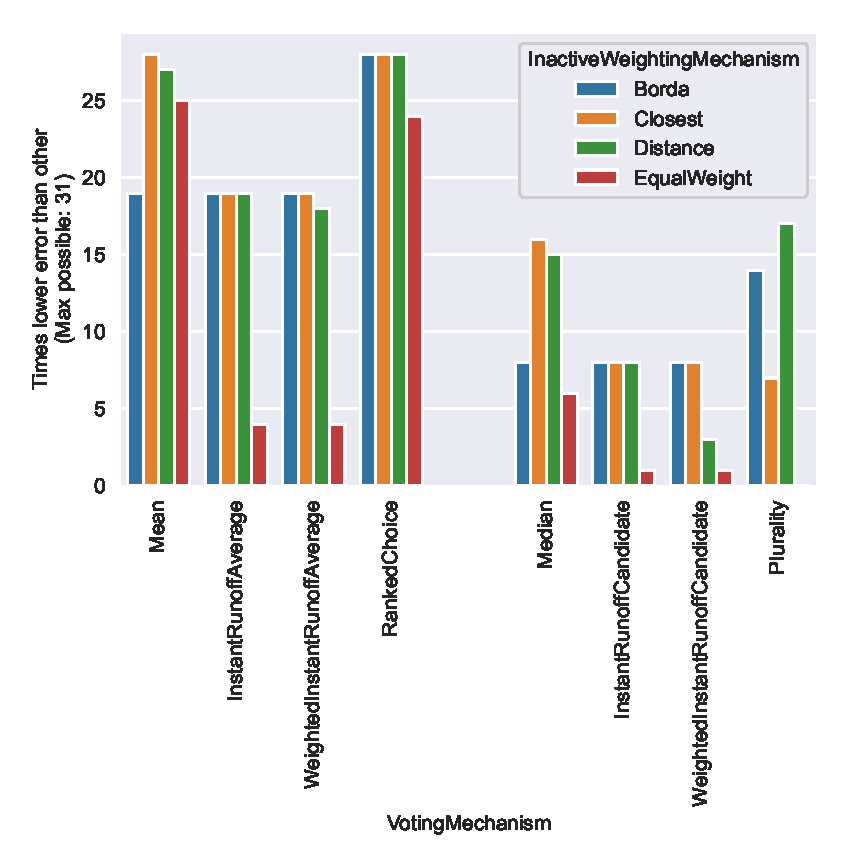
\includegraphics[scale=0.75]
    {./content/figures/combinations/combined_lesser_counts}
    \caption{The number of times each combination has a lower error according to
    U-tests.}
    \label{fig:combined-lesser_counts}
\end{figure}

From the graph, we can see our findings in~\fullref{sec:lowest-error-voting-mechanism}
hold true with the combinations as well, with Ranked Choice taking the top three ranks.
The rankings from~\fullref{sec:lowest-error-weighting-mechanism} also
generally hold true, since the Closest and Borda mechanisms generally
appear sooner than others.
It is possible, however, that voting mechanisms have a larger impact than weighting
mechanisms, since the general order of rankings more closely follows the voting
mechanism ordering rather than that of the weighting mechanisms.

%% I'm leaving this here in case I want to add it later. For now it seems like overkill
% Nevertheless, there may be occasions when candidate mechanisms may be preferable
% over average mechanisms, and so a deeper dive will be performed on both types of
% voting mechanisms.
%
% \subsection{Average Mechanisms}\label{subsec:lowest-error-combo-average}
%
% \subsection{Candidate Mechanisms}\label{subsec:lowest-error-combo-candidate}


\begin{table}[htbp]
    % increase table row spacing, adjust to taste
    \renewcommand{\arraystretch}{1.0}

    \caption{The rankings of combinations, ordered by the number of combinations
    beaten.
    The maximum number of combinations is 31 (32 total combinations, minus
    the combination being tested).
    Note that those with the same count are arranged in no particular order.}
    \label{tab:combined-overall-rankings}

    \centering
    \begin{tabular}{|c|c|c|}
        \hline
        Voting Mechanism                 & Weighting Mechanism & \# of Combos Beaten \\
        \hhline{|=|=|=|}
        Ranked Choice                    & Distance Voting     & 28                  \\
        \hline
        Ranked Choice                    & Closest             & 28                  \\
        \hline
        Ranked Choice                    & Borda               & 28                  \\
        \hline
        Mean                             & Closest             & 28                  \\
        \hline
        Mean                             & Distance Voting     & 27                  \\
        \hline
        Mean                             & Equal Weight        & 25                  \\
        \hline
        Ranked Choice                    & Equal Weight        & 24                  \\
        \hline
        Weight by Instant Runoff         & Borda               & 19                  \\
        \hline
        Averaged Weighted Instant Runoff & Borda               & 19                  \\
        \hline
        Weight by Instant Runoff         & Closest             & 19                  \\
        \hline
        Averaged Weighted Instant Runoff & Closest             & 19                  \\
        \hline
        Mean                             & Borda               & 19                  \\
        \hline
        Weight by Instant Runoff         & Distance Voting     & 19                  \\
        \hline
        Averaged Weighted Instant Runoff & Distance Voting     & 18                  \\
        \hline
        Plurality                        & Distance Voting     & 17                  \\
        \hline
        Median                           & Closest             & 16                  \\
        \hline
        Median                           & Distance Voting     & 15                  \\
        \hline
        Plurality                        & Borda               & 14                  \\
        \hline
        Weighted Instant Runoff          & Borda               & 8                   \\
        \hline
        Instant Runoff (Candidate)       & Distance Voting     & 8                   \\
        \hline
        Instant Runoff (Candidate)       & Closest             & 8                   \\
        \hline
        Instant Runoff (Candidate)       & Borda               & 8                   \\
        \hline
        Weighted Instant Runoff          & Closest             & 8                   \\
        \hline
        Median                           & Borda               & 8                   \\
        \hline
        Plurality                        & Closest             & 7                   \\
        \hline
        Median                           & Equal Weight        & 6                   \\
        \hline
        Averaged Weighted Instant Runoff & Equal Weight        & 4                   \\
        \hline
        Weight by Instant Runoff         & Equal Weight        & 4                   \\
        \hline
        Weighted Instant Runoff          & Distance Voting     & 3                   \\
        \hline
        Instant Runoff (Candidate)       & Equal Weight        & 1                   \\
        \hline
        Weighted Instant Runoff          & Equal Weight        & 1                   \\
        \hline
        Plurality                        & Equal Weight        & 0                   \\
        \hline
    \end{tabular}
\end{table}


\section{Weightlessly Averaging All Agents}\label{sec:weightless-average-all}
% Explain how WeightlessAverageAll works best
While the results thus far have been very interesting, the question of if using such
systems works better than simply averaging the estimates of all agents.
Such an operation is here dubbed `weightlessly averaging all,' since it ignores
weights and simply averages all agents, including inactive agents.
This technique does not use a weighting mechanism.
\autoref{fig:weightless-voting-mechanisms-comparison} shows how weightlessly
averaging all agents compares to the other mechanisms, ignoring which weighting
mechanism is used or the distribution of the proxies or inactive agents.

\begin{figure}[htbp]
    \centering
    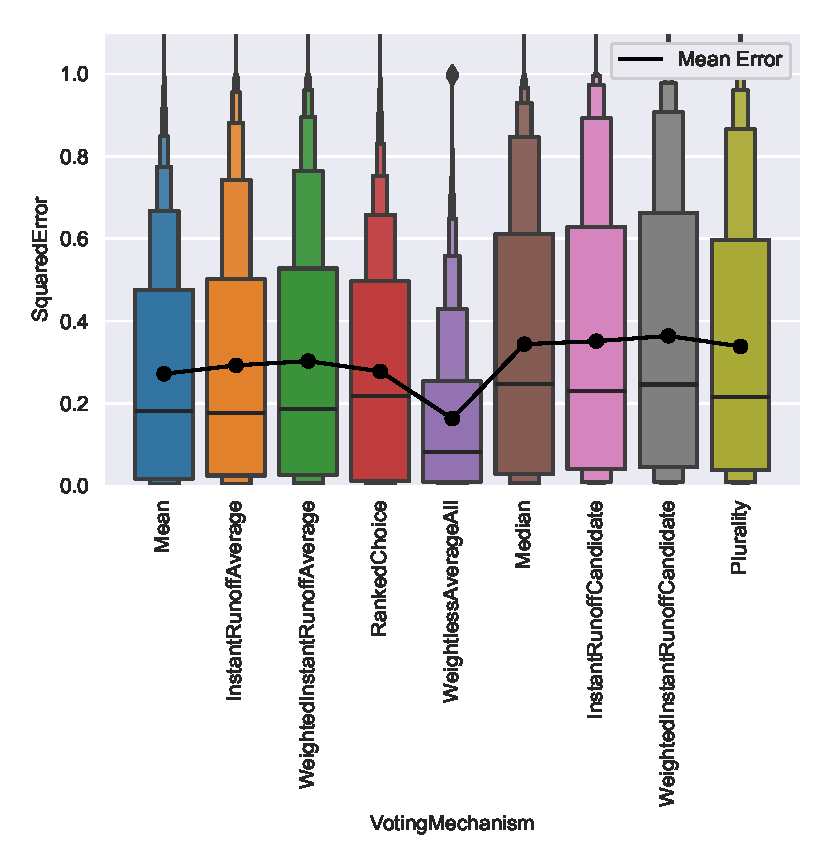
\includegraphics[scale=0.75]
    {./content/figures/weightless/weightless_voting_mechanisms_comparison}
    \caption{Squared error populations by voting mechanism, with average
    mechanisms on the left and candidate mechanisms on the right.
    Weightlessly averaging all agents' estimates is in the center.}
    \label{fig:weightless-voting-mechanisms-comparison}
\end{figure}

It is immediately evident that weightlessly averaging all agents' estimates works
considerable better that using proxy vote systems.
While this would initially indicate that proxy vote systems should not be used when a
simpler and more accurate technique already exists, this broad overview does not tell
the full story.
As explored previously, each voting mechanism is also paired with a weighting
mechanism that heavily influences its accuracy.
Additionally, we have yet to explore how the proxy and inactive estimate
distributions interact with the different mechanisms.

Indeed, performing tests on group separated by voting and weighting mechanisms as
well as proxy and inactive estimate distribution, indicates 467 of the 2048 possible
combinations, or 22.80\%, work better using a proxy vote system than weightlessly
averaging.
These tests are performed as if the proxy system was used instead of weightlessly
averaging, meaning that if the tests are performed groups with the same proxy and
inactive estimate distributions.

Of these 467 combinations, 223 (47.75\%) have an asymmetric proxy distribution with
a symmetric inactive distribution, while 154 (32.98\%) have an asymmetric inactive
distribution with a symmetric inactive distribution.
Additionally, 78 (16.70\%) use asymmetric distributions for both proxies and
inactive agents.
This totals to 455 (97.43\%) of the 467 more accurate proxy systems that use
asymmetric distributions!

The remaining 12 consist of high-performing voting mechanism/weighting mechanism
combinations, as discovered in \autoref{sec:lowest-error-overall-combination},
using Gaussian or \betadistribution{4}{4} distributions for the proxies,
and \betadistribution{0.3}{0.3} as the inactive distributions.
These combinations are displayed in~\autoref{tab:non-asymmetric-lower-pop-systems}.

\begin{table}[htbp]
    % increase table row spacing, adjust to taste
    \renewcommand{\arraystretch}{1.0}

    \caption{The proxy voting systems that still achieve a lower error than
    weightless average all, in no particular order.}
    \label{tab:non-asymmetric-lower-pop-systems}

    \centering
    \begin{tabular}{|c|c|c|c|}
        \hline
        Voting Mechanism & %
        Weighting Mechanism & %
        Proxy Distribution & %
        Inactive Distribution \\
        \hhline{|=|=|=|=|}
        Mean & Borda & \betadistribution{4}{4} & \betadistribution{0
        .3}{0.3} \\
        \hline
        Mean & Equal Weight & \betadistribution{4}{4} & \betadistribution{0
        .3}{0.3} \\
        \hline
        Mean & Borda & Gaussian & \betadistribution{0
        .3}{0.3} \\
        \hline
        Mean & Distance & Gaussian & \betadistribution{0
        .3}{0.3} \\
        \hline
        Mean & Equal Weight & Gaussian & \betadistribution{0
        .3}{0.3} \\
        \hline
        Ranked Choice & Borda & \betadistribution{4}{4} & \betadistribution{0
        .3}{0.3} \\
        \hline
        Ranked Choice & Closest & \betadistribution{4}{4} & \betadistribution{0
        .3}{0.3} \\
        \hline
        Ranked Choice & Distance & \betadistribution{4}{4} & \betadistribution{0
        .3}{0.3} \\
        \hline
        Ranked Choice & Borda & Gaussian & \betadistribution{0
        .3}{0.3} \\
        \hline
        Ranked Choice & Closest & Gaussian & \betadistribution{0
        .3}{0.3} \\
        \hline
        Ranked Choice & Distance & Gaussian & \betadistribution{0
        .3}{0.3} \\
        \hline
        Ranked Choice & Equal Weight & Gaussian & \betadistribution{0
        .3}{0.3} \\
        \hline
    \end{tabular}
\end{table}

However, this does not mean a proxy system is always better when some distribution is
asymmetrical.
The number of lower error asymmetric combinations is only 29.62\% of the 1536
possible combinations with at least one distribution asymmetric, and all 467 lower error
combinations are only 22.80\% of all 2048 combinations.
Ten combinations with at least one asymmetric distribution failed to achieve a lower
error, regardless of the mechanism used.
These combinations are shown in \autoref{tab:no-appearance-distro-combos}.
Of note is in all these combinations, both distributions are asymmetric.
Additionally, whenever an asymmetric distribution is placed with itself, a proxy system
does not produce a lower error.
Finally, the more heavily skewed asymmetric distributions work worse with other
asymmetric distributions.

\begin{table}[htbp]
    % increase table row spacing, adjust to taste
    \renewcommand{\arraystretch}{1.0}

    \caption{The asymmetric distribution combinations that were never found to achieve
    lower error than weightlessly averaging, arranged in no particular order.}
    \label{tab:no-appearance-distro-combos}

    \centering
    \begin{tabular}{|c|c|}
        \hline
        Proxy Distribution        & Inactive Distribution     \\
        \hhline{|=|=|}
        \betadistribution{0.3}{3} & \betadistribution{0.3}{3} \\
        \hline
        \betadistribution{0.3}{3} & \betadistribution{3}{0.3} \\
        \hline
        \betadistribution{0.3}{3} & \betadistribution{4}{1}   \\
        \hline
        \betadistribution{1}{4}   & \betadistribution{1}{4}   \\
        \hline
        \betadistribution{1}{4}   & \betadistribution{4}{1}   \\
        \hline
        \betadistribution{3}{0.3} & \betadistribution{0.3}{3} \\
        \hline
        \betadistribution{3}{0.3} & \betadistribution{1}{4}   \\
        \hline
        \betadistribution{3}{0.3} & \betadistribution{3}{0.3} \\
        \hline
        \betadistribution{4}{1}   & \betadistribution{1}{4}   \\
        \hline
        \betadistribution{4}{1}   & \betadistribution{4}{1}   \\
        \hline
    \end{tabular}
\end{table}

A natural next question is which mechanism combinations are more likely to produce a
lower error?
The count of how many times each voting mechanism/weighting mechanism combination
tests to have a lower error than weightlessly averaging in displayed
in~\autoref{tab:lower-pop-combo-count}.
This table would seem to indicate that the stronger combinations are more able to
achieve a lower error.
Surprisingly, even candidate mechanisms are occasionally able to achieve a lower error
as well.

\begin{table}[htbp]
    % increase table row spacing, adjust to taste
    \renewcommand{\arraystretch}{1.0}

    \caption{The count of mechanism combinations the achieve a lower error
    population than weightlessly averaging, ordered by count, then voting mechanism,
        and finally weighting mechanism.}
    \label{tab:lower-pop-combo-count}

    \centering
    \begin{tabular}{|c|c|c|}
        \hline
        Voting Mechanism                    & Weighting Mechanism & Count \\
        \hhline{|=|=|=|}
        Mean                                & Equal Weight        & 20    \\
        \hline
        Plurality                           & Closest             & 20    \\
        \hline
        Ranked Choice                       & Borda               & 20    \\
        \hline
        Ranked Choice                       & Closest             & 20    \\
        \hline
        Ranked Choice                       & Distance            & 20    \\
        \hline
        Ranked Choice                       & Equal Weight        & 19    \\
        \hline
        Instant Runoff (Average)            & Borda               & 16    \\
        \hline
        Instant Runoff (Average)            & Closest             & 16    \\
        \hline
        Instant Runoff (Average)            & Distance            & 16    \\
        \hline
        Mean                                & Borda               & 16    \\
        \hline
        Mean                                & Closest             & 16    \\
        \hline
        Median                              & Closest             & 16    \\
        \hline
        Weighted Instant Runoff (Average)   & Borda               & 16    \\
        \hline
        Weighted Instant Runoff (Average)   & Closest             & 16    \\
        \hline
        Instant Runoff (Average)            & Equal Weight        & 14    \\
        \hline
        Instant Runoff (Candidate)          & Borda               & 14    \\
        \hline
        Instant Runoff (Candidate)          & Closest             & 14    \\
        \hline
        Instant Runoff (Candidate)          & Distance            & 14    \\
        \hline
        Median                              & Equal Weight        & 14    \\
        \hline
        Plurality                           & Distance            & 14    \\
        \hline
        Weighted Instant Runoff (Average)   & Equal Weight        & 14    \\
        \hline
        Weighted Instant Runoff (Candidate) & Borda               & 14    \\
        \hline
        Weighted Instant Runoff (Candidate) & Closest             & 14    \\
        \hline
        Instant Runoff (Candidate)          & Equal Weight        & 13    \\
        \hline
        Weighted Instant Runoff (Candidate) & Equal Weight        & 13    \\
        \hline
        Mean                                & Distance            & 11    \\
        \hline
        Plurality                           & Equal Weight        & 11    \\
        \hline
        Median                              & Borda               & 10    \\
        \hline
        Weighted Instant Runoff (Average)   & Distance            & 10    \\
        \hline
        Weighted Instant Runoff (Candidate) & Distance            & 10    \\
        \hline
        Median                              & Distance            & 8     \\
        \hline
        Plurality                           & Borda               & 8     \\
        \hline
    \end{tabular}
\end{table}

While it is clear that simply weightlessly averaging all agent's estimates is a more
accurate method, there appear to be occasions when proxy vote systems can reduce
error, particularly when one of the error distributions is asymmetrical.
This look into distributions and other parameters begs for a closer look and may yield
fascinating results upon closer inspection.

\section{How many Agents to Use}\label{sec:how-many-agents}
Regardless of which combination of mechanisms is used, the question still remains,
`How many proxies and inactive agents should be used?'
This question directly affects the cost of a system, since the cost is tied to the
number of agents, and so ideally the number of agents should be minimized.

There are three parts to this question, all of which will be addressed here.
The first is how many proxies should be used.
\autoref{fig:proxy-count} shows how proxy count affects the error of a system.
From this graph, we can see in the beginning more proxies produces better results.
However, this benefit reduces over time and eventually flattens out or, in the case
of some combinations, increases the error of a system.
This benefit seems to bottom out between 10 and 15 proxies.

\begin{figure}[htbp]
    \centering
    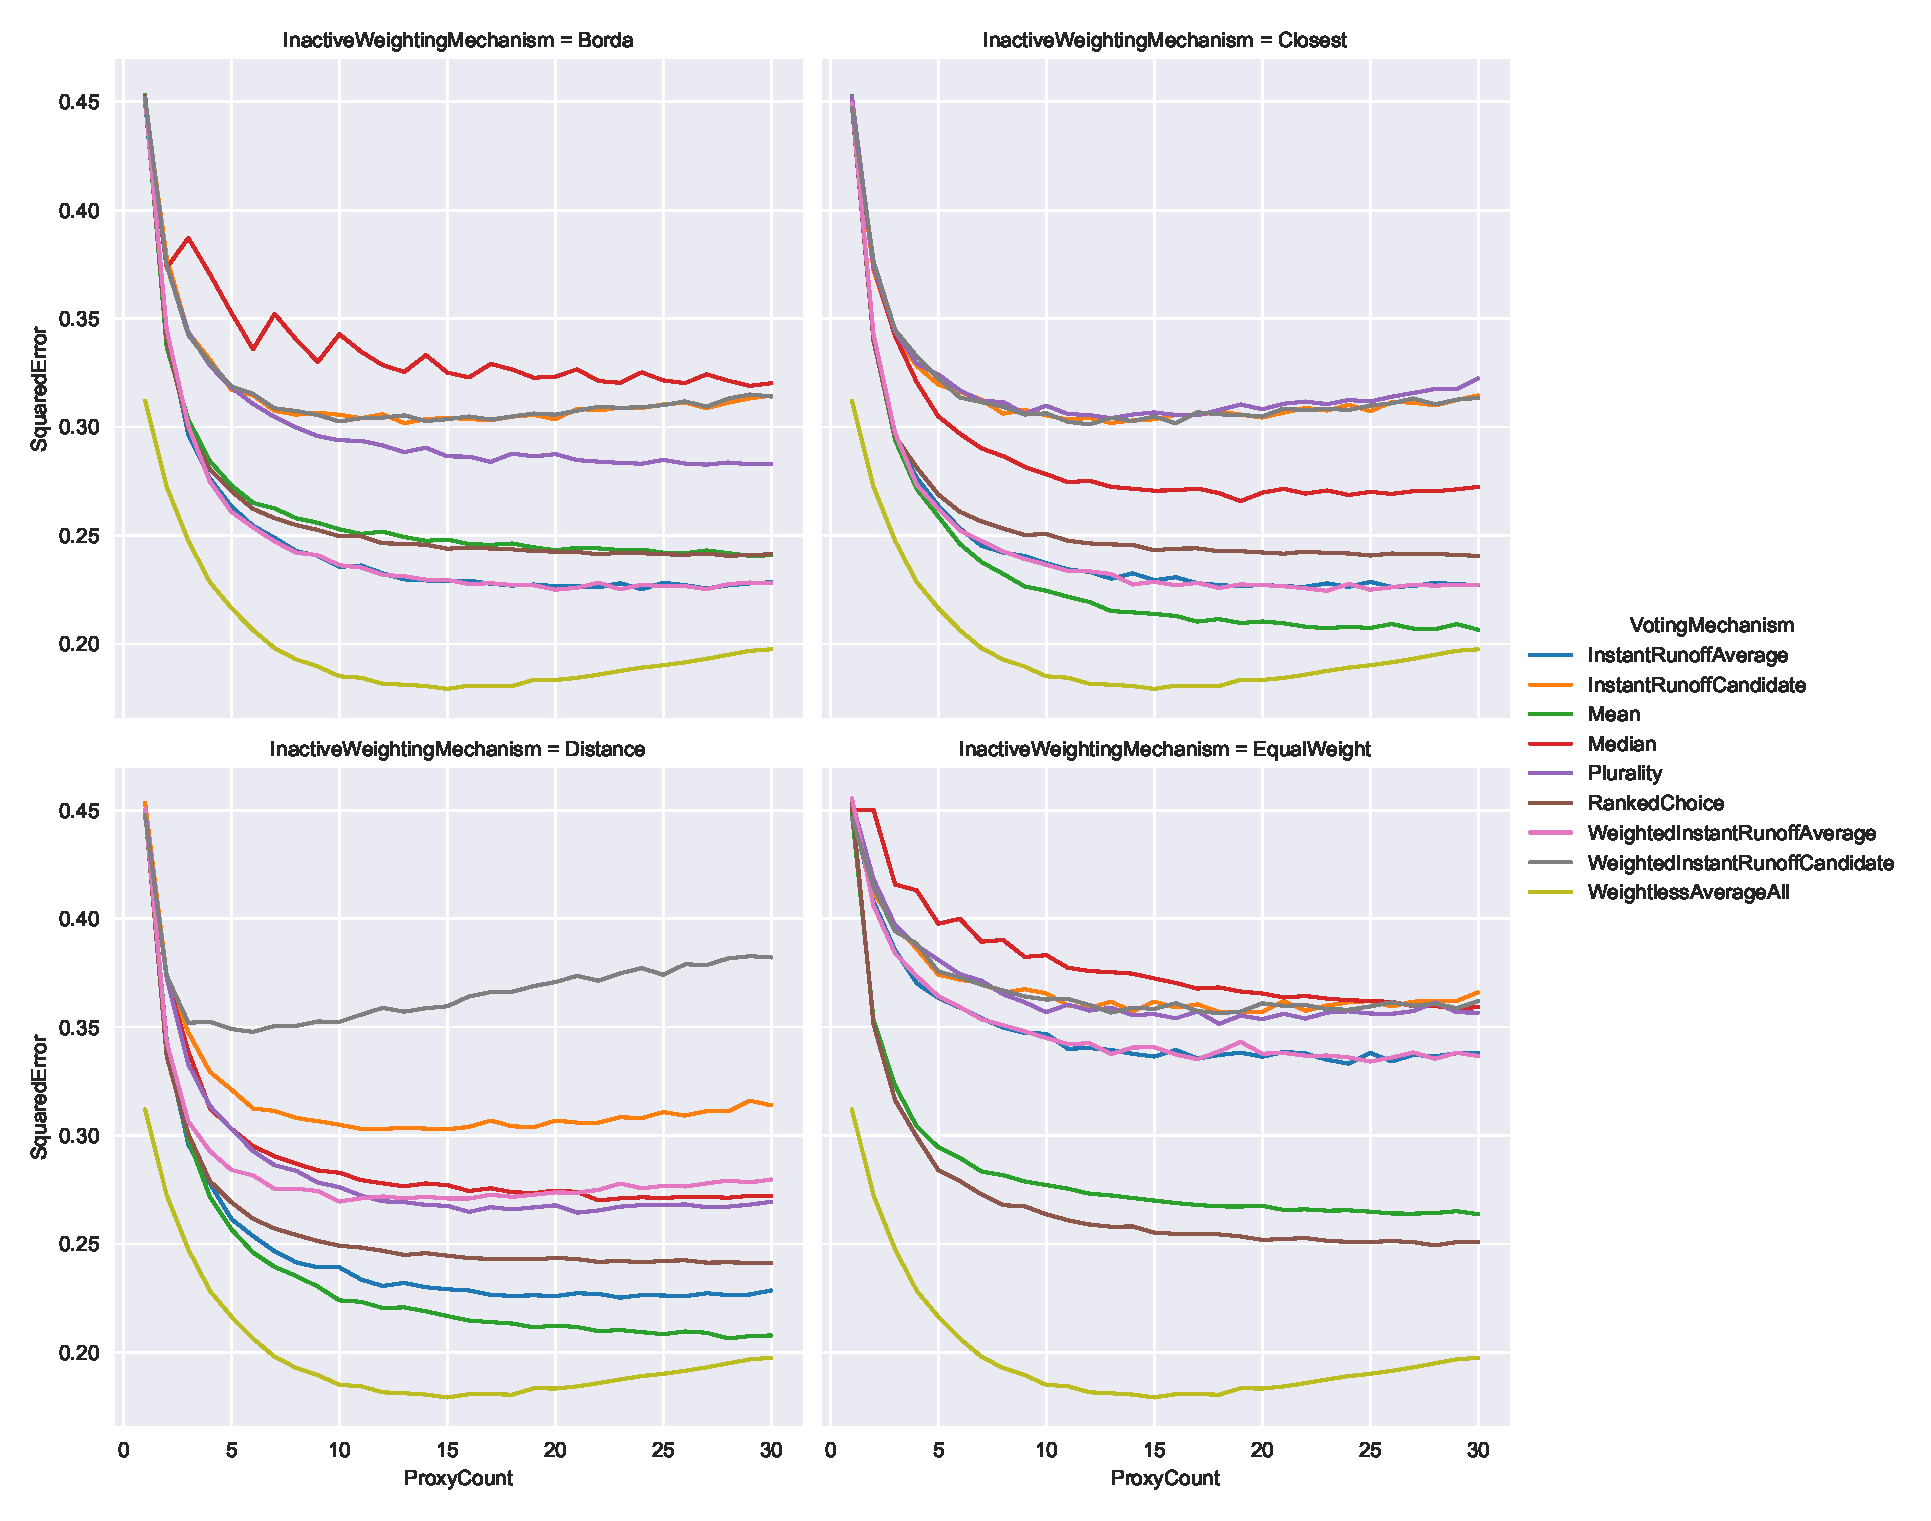
\includegraphics[
        width=\textwidth,
        height=\dimexpr
        \textheight - 4 % Could also be .9\textheight
        \baselineskip,
        keepaspectratio]
    {./content/figures/ratios/proxy_count}
    \caption{How the number of proxies affects the system error.}
    \label{fig:proxy-count}
\end{figure}

The second part of determining how many agents to use is how many inactive agents to
use.
As with minimizing the number of proxies, minimizing the number of inactive agents to
use will help reduce the costs of the system.
\autoref{fig:inactive-count} seems to indicate that, with the exception of
weightlessly averaging all agents, there is little benefit in using more inactive
agents.
This doesn't mean only one inactive agent should be used, as is indicated by the
third part of the question: the ratio between proxies and inactive agents.

\begin{figure}[htbp]
    \centering
    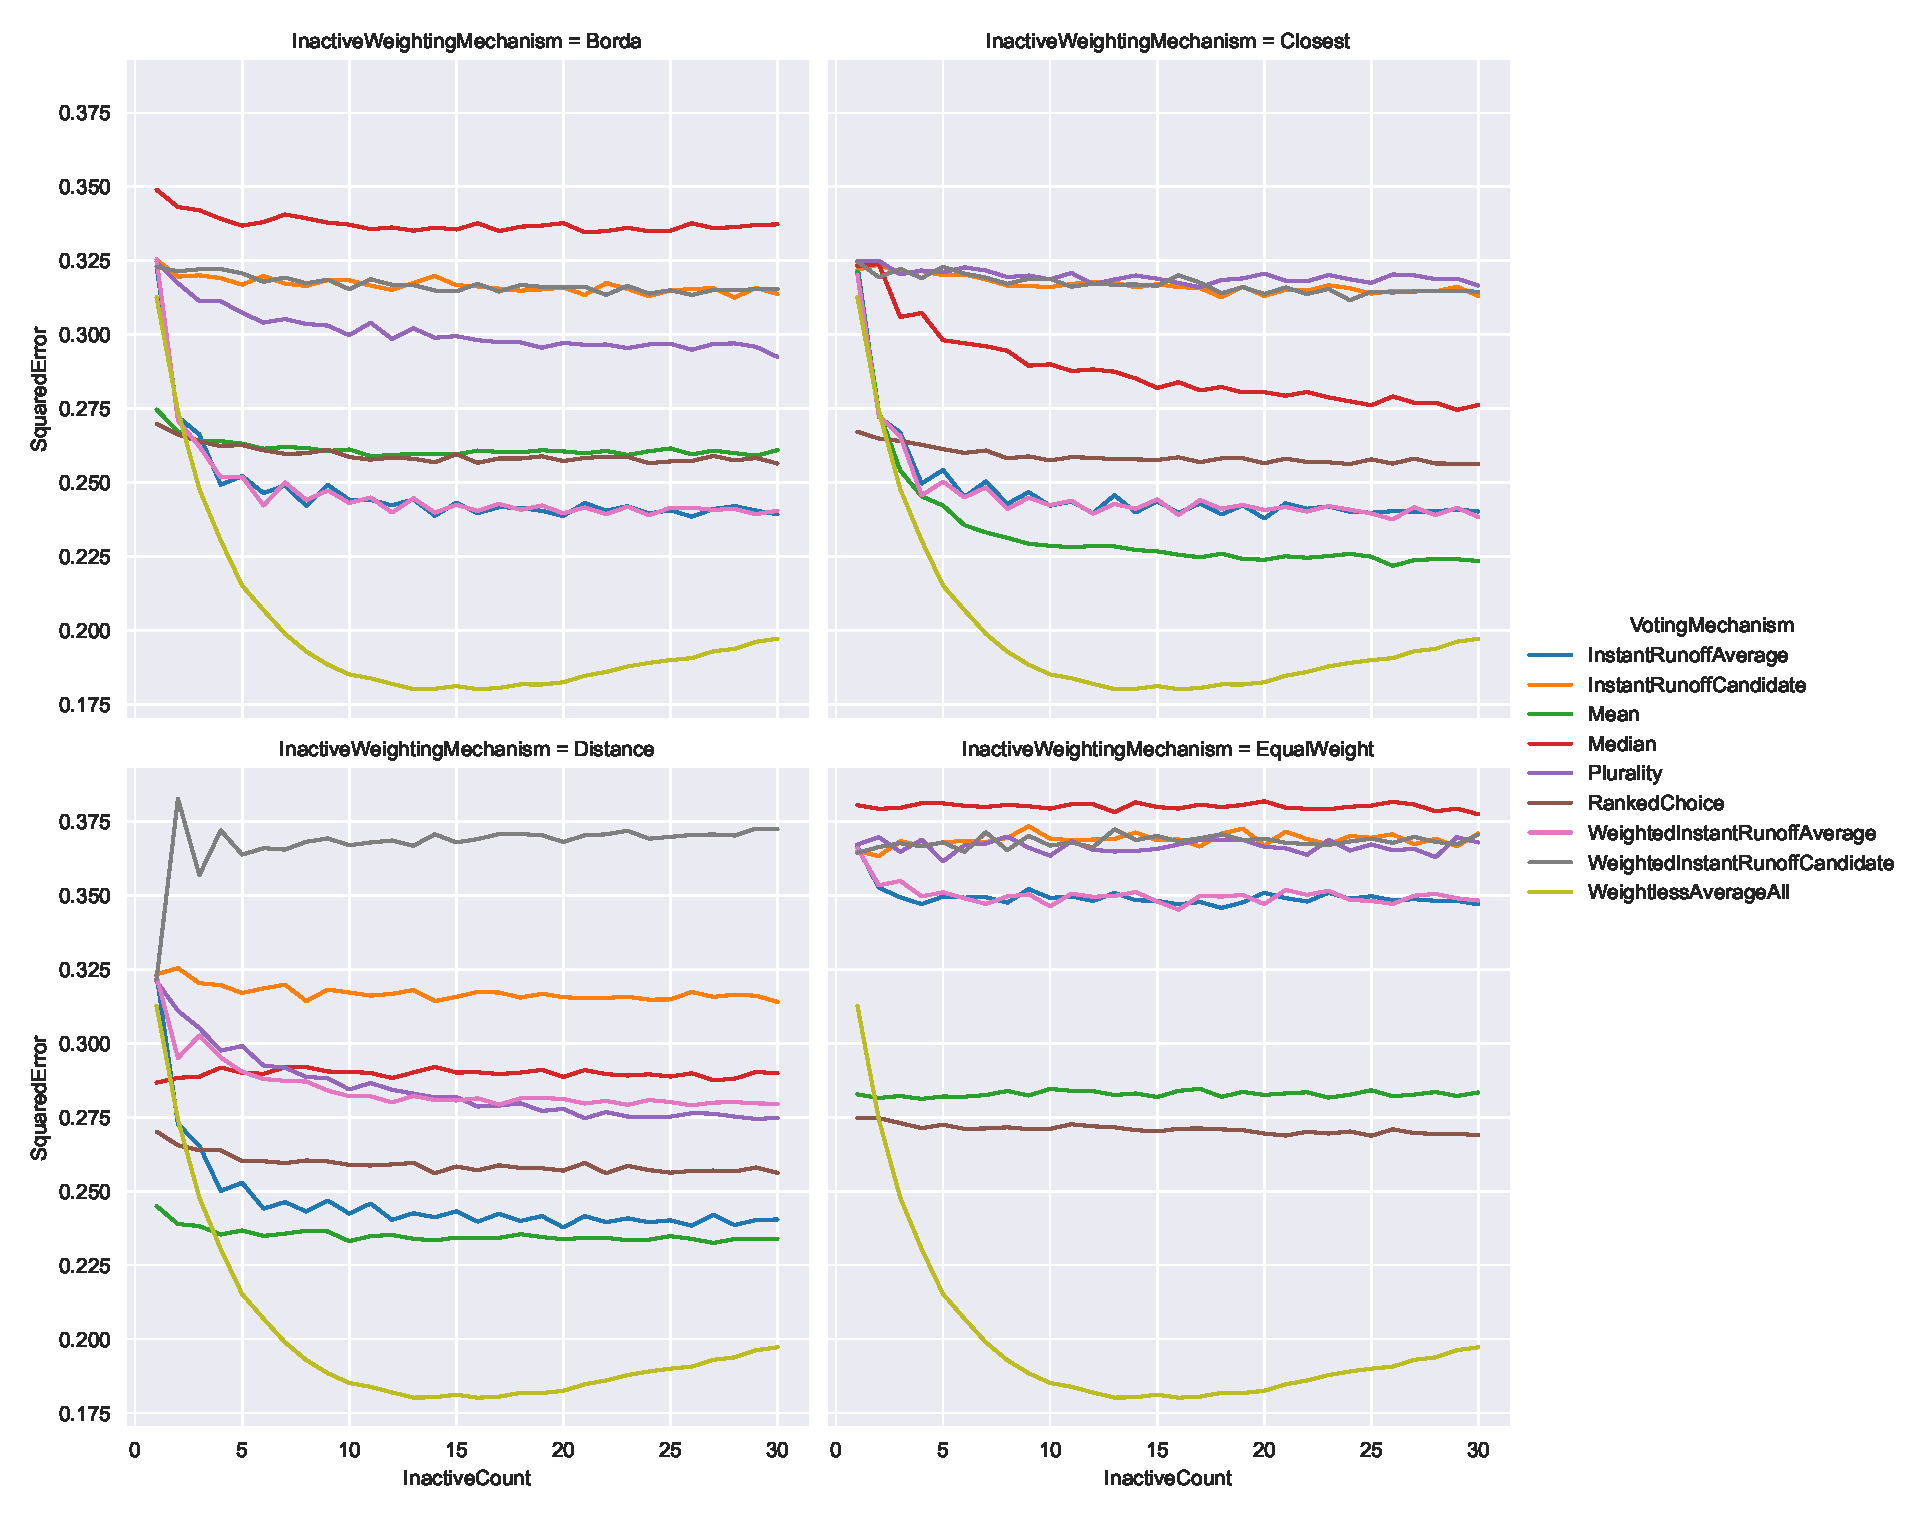
\includegraphics[
        width=\textwidth,
        height=\dimexpr
        \textheight - 4 % Could also be .9\textheight
        \baselineskip,
        keepaspectratio]
    {./content/figures/ratios/inactive_count}
    \caption{How the number of inactive agents affects the system error.}
    \label{fig:inactive-count}
\end{figure}

\autoref{fig:ratios}~and~\ref{fig:ratios-zoomed} display the error in the system as
the ratio between proxies and inactive agents increases, with
\autoref{fig:ratios-zoomed} providing a zoomed-in perspective.
Interestingly, the curve produced in each of these graphs flattens around a 1:1
ratio, indicating that there is little or no benefit to having a differing number of
proxies and inactive agents.
Additionally, there seems to be small `hiccups' at each whole number.
While the reason for this is not explored in this study, this would indicate that
slightly higher or lower ratio than 1:1 should be used.
With this mind, and since the number of inactive agents generally does not have an
effect on the system error, it would likely be best to use slightly fewer inactive
agents than proxy agents in an effort to decrease the total system cost and increase
system accuracy.

\begin{figure}[htbp]
    \centering
    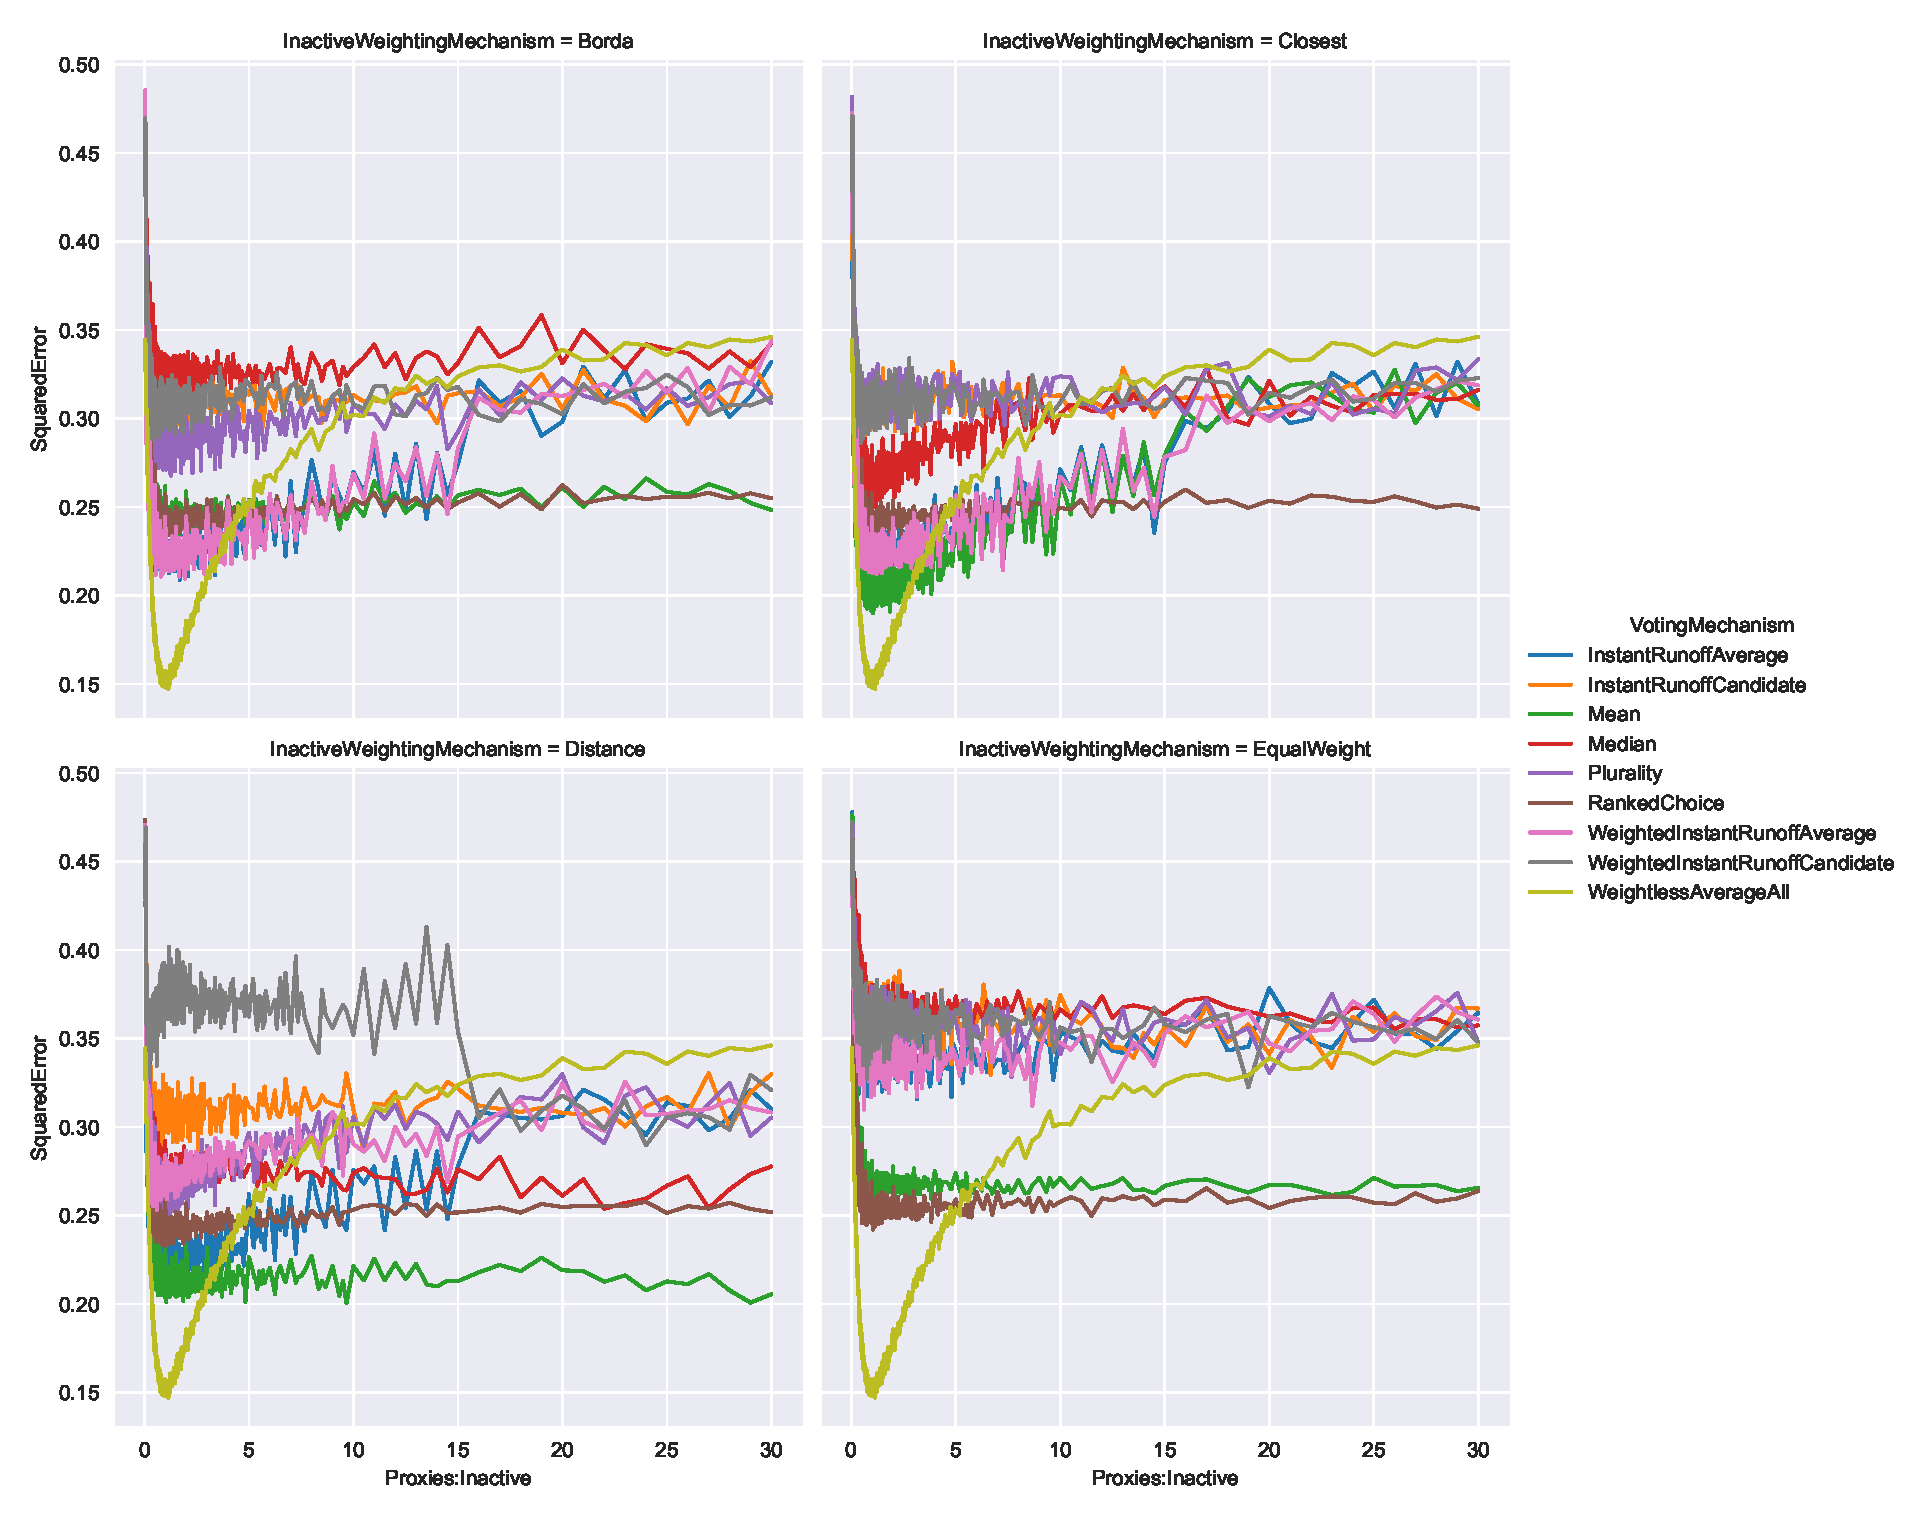
\includegraphics[
        width=\textwidth,
        height=\dimexpr
        \textheight - 4 % Could also be .9\textheight
        \baselineskip,
        keepaspectratio]
    {./content/figures/ratios/ratios}
    \caption{How the ratio between proxies and inactive agents affects the system
    error.}
    \label{fig:ratios}
\end{figure}

\begin{figure}[htbp]
    \centering
    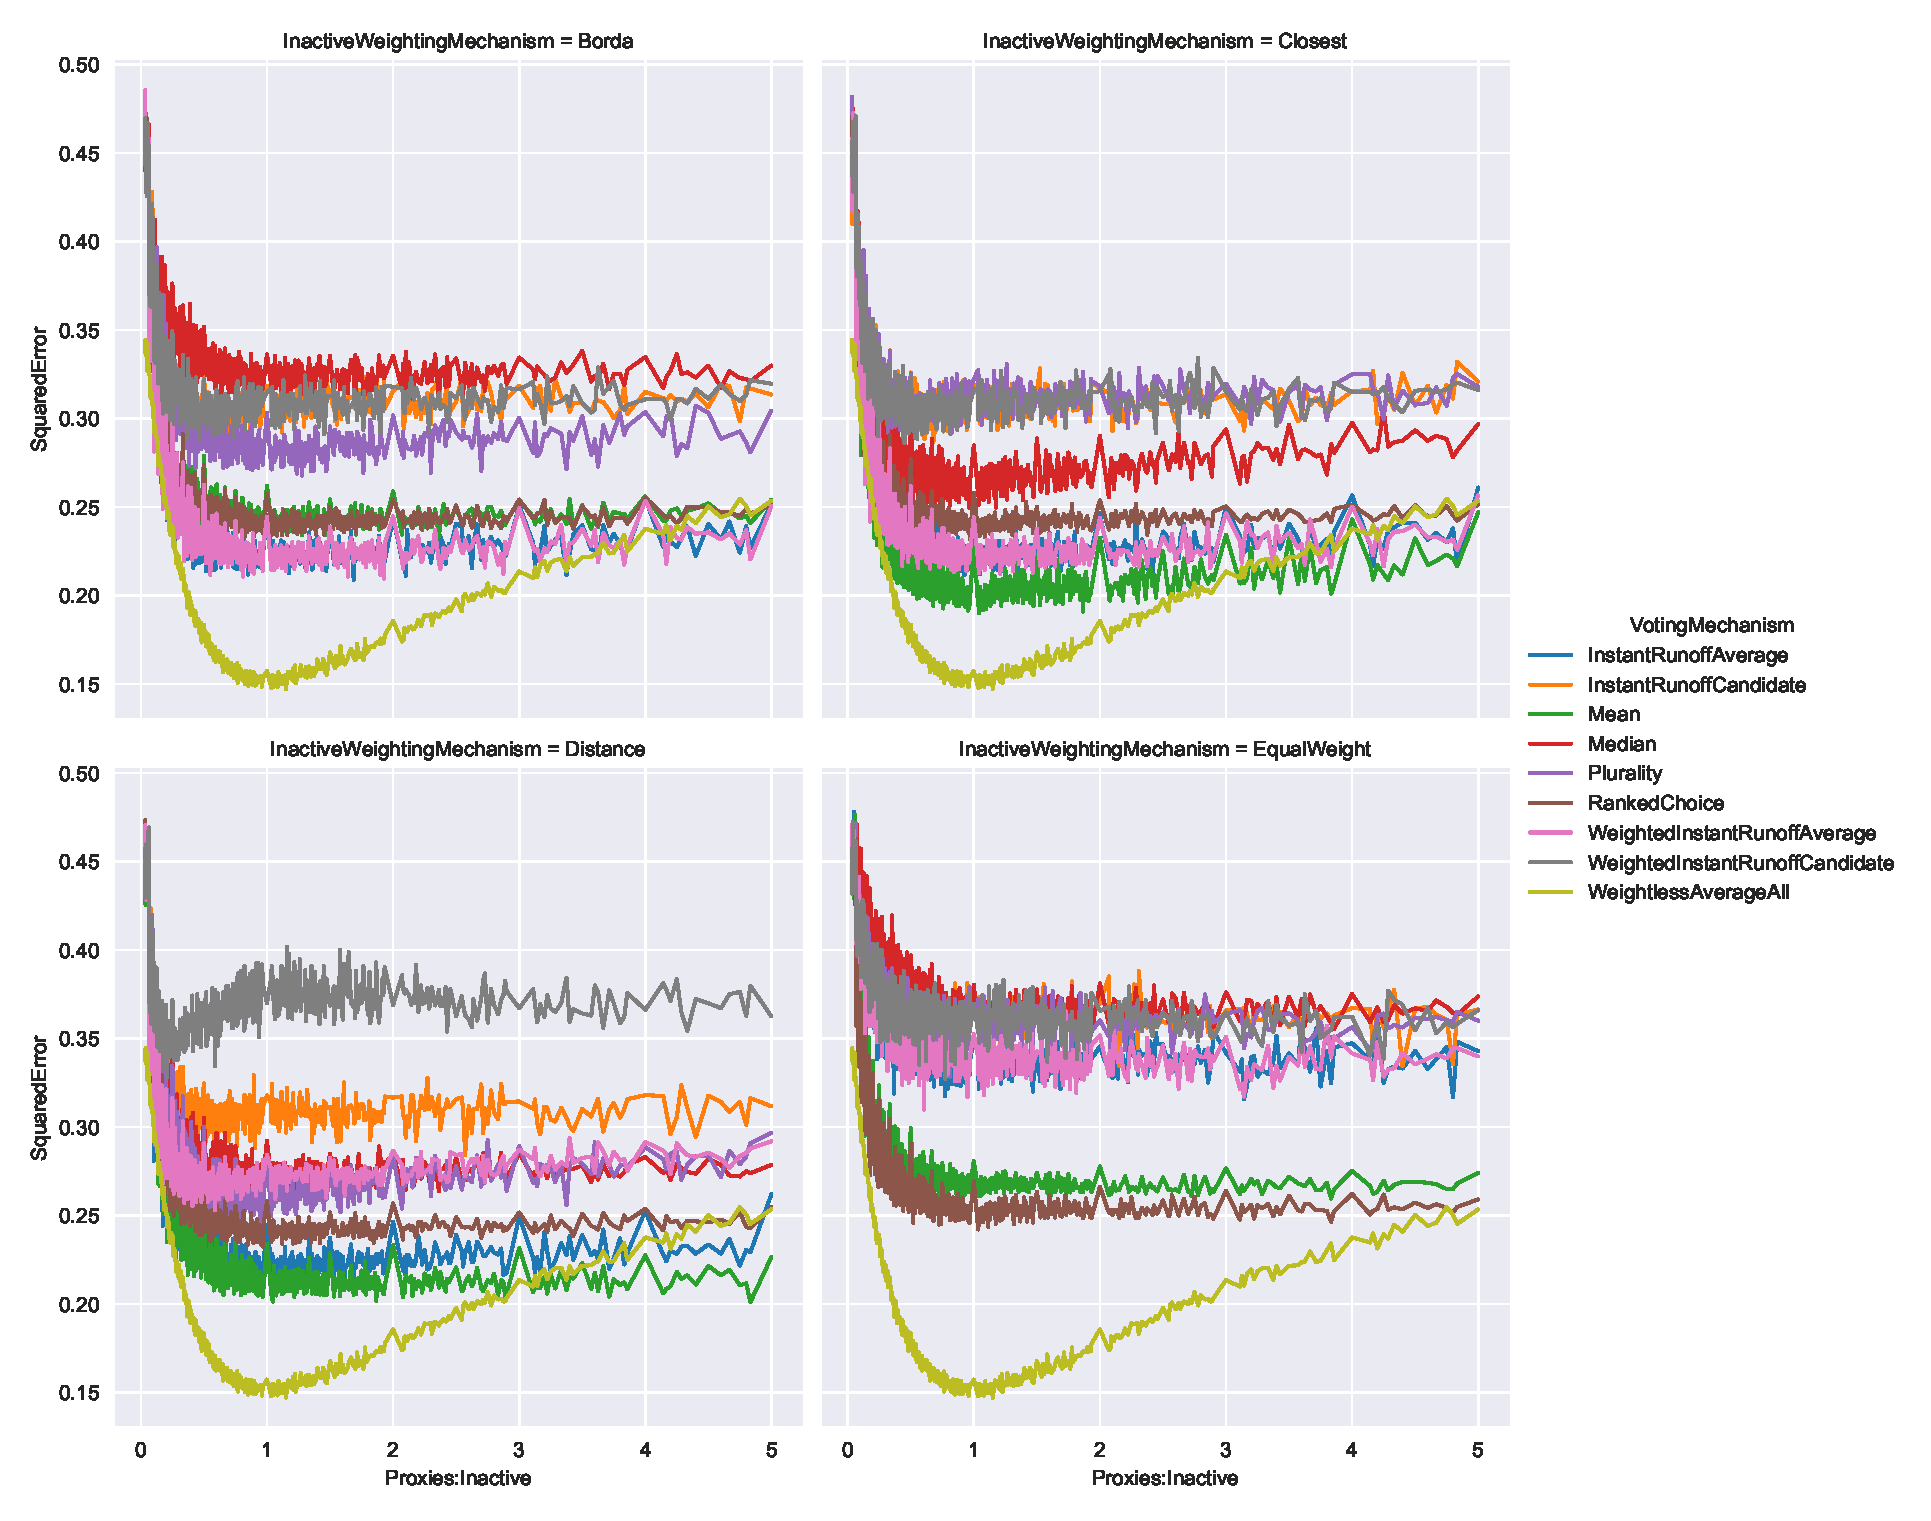
\includegraphics[
        width=\textwidth,
        height=\dimexpr
        \textheight - 4 % Could also be .9\textheight
        \baselineskip,
        keepaspectratio]
    {./content/figures/ratios/ratios_zoomed}
    \caption{How the ratio between proxies and inactive agents affects the system
    error. Zoomed in to better see the curve.}
    \label{fig:ratios-zoomed}
\end{figure}
